\newpage
 \begin{center}
 \begin{Large}
 \textbf{
% Gaussian Process Dynamical Systems\\
 Appendix
 } \\
 \end{Large}
% \noindent \newline
% \textbf{Andreas Damianou, Michalis Titsias, Neil Lawrence}
 \end{center}
\appendix
\section{Derivation of the variational bound}

We wish to approximate the marginal likelihood:
\begin{equation}
\label{marginalLikelihoodSuppl}
p(Y | \bft) =  \int p( Y , F, X| \bft) \intd  X \intd F,
\end{equation}
by computing a lower bound:
\begin{align}
\mathcal{F}_v(q, \boldsymbol \theta) = {}& \int q(\mathit{\Theta}) \log 
		\frac{ p(Y , F , \mathit{X} | \mathbf{t})}
			 {q(\mathit{\Theta})}  \intd  X \intd F.
% 	    \nonumber \\
% 	      = {}& \sum_{d=1}^D \int q(\Theta) \log \left( p(\bfy_d | \bff_d) p(\bff_d | X) \right) dX d \bff_d -
% 		    \int q(\Theta) \frac{p(X|\bft)}{q(\Theta)} dX
		 \label{jensens1Suppl}
\end{align}
%
This can be achieved by first augmenting the joint probability density of our model with inducing inputs $\tilde{X}$ along with their corresponding function values $U$:
\begin{equation}
 \label{augmentedJointSuppl}
p(Y,F, U,X,\tilde{X} | \bft) = \prod_{d=1}^D p(\mathbf{y}_d | \mathbf{f}_d) p(\mathbf{f}_d | \mathbf{u}_d, \mathit{X})
p(\bfu_d | \tilde{X})  p(X | \mathbf{t})
\end{equation}
where $p(\bfu_d | \tilde{X}) = \prod_{d=1}^D \mathcal{N} \left( \bfu_d | \mathbf{0}, K_{MM} \right)$ . For simplicity, $\tilde{X}$ is dropped from our
expressions for the rest of this supplementary material. Note that after including the inducing points, $p(\bff_d | \bfu_d, X)$
remains analytically tractable and it turns out to be \cite{rasmussen-williams}):
\begin{equation}
 \label{priorF2Suppl}
p(\bff_d | \bfu_d, X) =  \mathcal{N}  \left( \bff_d | K_{NM} K_{MM}^{-1} \bfu_d , K_{NN} - K_{NM} K_{MM}^{-1} K_{MN} \right).
\end{equation}
For tractability, we now define a variational density $q(\Theta)$:
\begin{equation}
\label{varDistrSuppl}
q(\mathit{\Theta}) = q(F, U,X) = q(F | U, X) q(U) q(X) = \prod_{d=1}^D p(\bff_d | \bfu_d, X )q(\bfu_d) q(X),
\end{equation}
%
%
where $q(X) = \prod_{q=1}^Q \mathcal{N} \left( \bfx_q | \bfmu_q, S_q \right)$. 
%
Now, we return to \eqref{jensens1Suppl} and replace the joint distribution with its augmented version \eqref{augmentedJointSuppl} and the variational distribution with its factorised version \eqref{varDistrSuppl}:
\begin{align}
\mathcal{F}_v(q, \boldsymbol \theta) = {}& \int q(\mathit{\Theta}) \log 
		\frac{ p(Y,F, U,X | \bft)}
			 {q(F, U,X)}  \intd  X \intd F,
 	    \nonumber \\
= {}& \int \prod_{d=1}^D p(\bff_d | \bfu_d, X )q(\bfu_d) q(X) 
	    \log  \frac{\prod_{d=1}^D p(\mathbf{y}_d | \mathbf{f}_d) \cancel{p(\mathbf{f}_d | \mathbf{u}_d, \mathit{X})}
						p(\bfu_d | \tilde{X})  p(X | \mathbf{t})}
 	      		   {\prod_{d=1}^D \cancel{p(\bff_d | \bfu_d, X )}q(\bfu_d) q(X)}   \intd  X \intd F \nonumber \\
= {}& \int \prod_{d=1}^D p(\bff_d | \bfu_d, X )q(\bfu_d) q(X) 
		\log  \frac{\prod_{d=1}^D p(\mathbf{y}_d | \mathbf{f}_d) p(\bfu_d | \tilde{X})}
				   {\prod_{d=1}^D q(\bfu_d) q(X)}   \intd  X \intd F \nonumber \\
- {}& \int \prod_{d=1}^D  q(X)   \log \frac{q(X)}{p(X | \mathbf{t})}   \intd  X \nonumber \\
= {}& \hat{\mathcal{F}}_v - \text{KL}(q \parallel p), \label{jensensSuppl}
\end{align}
%
with:
 \begin{equation}
\hat{\mathcal{F}}_v = 
\sum_{d=1}^D \left( 
    \int q(\bfu_d) q(X) \left\langle \log p(\bfy_d | \bff_d) \right\rangle_{p(\bff_d | \bfu_d, X)} d\bfu_d \; dX +
					   \log \left\langle \frac{p(\bfu_d)}{q(\bfu_d)} \right\rangle_{q(\bfu_d)} 
  \right) = \sum_{d=1}^D \hat{\mathcal{F}}_d
\end{equation} 

Both terms in \eqref{jensensSuppl} are analytically tractable, with the first having the same analytical solution as the one derived in \cite{BayesianGPLVM}. Further calculations in the the $\hat{\mathcal{F}}_v$ term reveal that the optimal setting for $q(\bfu_d)$ is also a Gaussian. More specifically, 
we have:
\begin{align}
\hat{\mathcal{F}}_v={}& \int q(\bfu_d) \log \frac{e^{\la \log N \left( \bfy_d | \bfa_d, \beta^{-1} I_d \right) \ra_{q(X)}}
		p(\bfu_d)}{q(\bfu_d)} d\bfu_d - A \label{boundFAnalytically5}
\end{align}
where $A$ is a collection of remaining terms and $\bfa_d$ is the mean of \eqref{priorF2Suppl}.
\eqref{boundFAnalytically5} is a KL-like quantity and, therefore, $q(\bfu_d)$ is optimally set to be the quantity appearing in the numerator of the above equation. So:
%:
% \begin{equation}
% q(\bff_{*,d}^m | X_*) = \mathcal{N}(\bff_{*,d}^m| \beta K_{N_* M} 
% (K_{MM} + \beta \Psi_2)^{-1} \Psi_1^{T} \bfy_d, K_{N_* N_*} - 
%  K_{N_* M} \left[ K_{M M}^{-1}  - (K_{M M} + \beta \Psi_2)^{-1} \right] 
%  K_{N_* M}^{T}),
% \end{equation}
% exactly as in \cite{BayesianGPLVM}.
\begin{equation}
\label{qu}
q(\bfu_d) = e^{\la \log \mathcal{N} \left( \bfy_d | \bfa_d, \beta^{-1} I_d \right) \ra_{q(X)}}
		p(\bfu_d) ,
\end{equation}
exactly as in \cite{BayesianGPLVM}. This is a Gaussian distribution since $p(\bfu_d ) = \mathcal{N} (\bfu_d | \mathbf{0}, K_{MM} )$.

\par
The complete form of the Jensen's lower bound turns out to be:
\begin{align}
\mathcal{F}_v(q, \boldsymbol \theta) = {}& \sum_{d=1}^{D} 
	\hat{\mathcal{F}}_d(q, \boldsymbol \theta) -  \text{KL}(q \parallel p) \nonumber \\
	= {}& 
	\sum_{d=1}^{D} 
		\log \left( 
		\frac{(\beta)^{\frac{N}{2}} \vert \mathit{K_{MM}} \vert ^\frac{1}{2} }
			 {(2\pi)^{\frac{N}{2}} \vert \beta \Psi_2 + \mathit{K_{MM}}  \vert ^\frac{1}{2} } 	
		 e^{-\frac{1}{2} \mathbf{y}^{T}_{d} W \mathbf{y}_d} 
		 \right) -
		 \frac{\beta \psi_0}{2} + \frac{\beta}{2} 
		 \text{Tr} \left( \mathit{K_{MM}^{-1}} \Psi_2 \right)  \nonumber \\
{}&	- \frac{Q}{2} \log \vert \mathit{K_t} \vert - \frac{1}{2} \sum_{q=1}^{Q}
	  \left[ \text{Tr} \left( \mathit{K_t}^{-1} \mathit{S_q} \right)	  
	  	   + \text{Tr} \left( \mathit{K_t}^{-1} \boldsymbol \mu_q \boldsymbol \mu_q^T \right) \right] 
	 + \frac{1}{2} \sum_{q=1}^Q \log \vert \mathit{S_q} \vert + const  \label{boundFinal}
\end{align}
where the last line corresponds to the KL term. Also:
\begin{equation}
\label{psis}
\Psi_0 = \text{Tr}(\langle \mathit{K_{NN}} \rangle_{q(\mathit{X})}) \;, \;\;
\Psi_1 = \langle \mathit{K_{NM}} \rangle_{q(\mathit{X})} \;, \;\;
\Psi_2 = \langle \mathit{K_{MN}} \mathit{K_{NM}} \rangle_{q(\mathit{X})}
\end{equation}
The $\Psi$ quantities can be computed analytically as in \cite{BayesianGPLVM}.


%-------------------------

\section{Derivatives of the variational bound}
Before giving the expressions for the derivatives of the variational bound \eqref{jensensSuppl},
it should be reminded that the variational parameters $\mu_q$ and $S_q$ (for all $q$s) have been
reparametrized as $S_q = \left( \mathit{K}_t^{-1} + diag(\boldsymbol \lambda_q) \right)^{-1}  \text{ and }   \boldsymbol \mu_q = K_t \bar{\boldsymbol \mu}_q$, where the function $diag(\cdot)$ transforms a vector into a square diagonal matrix and vice versa. Given the above, the set of the parameters to be optimised is 
$( \boldsymbol \theta_f, \boldsymbol \theta_x, \{ \bar{\bfmu}_q, \boldsymbol \lambda_q \}_{q=1}^Q, \tilde{X})$. The gradient w.r.t the inducing points $\tilde{X}$, however, has exactly the same form as for $\boldsymbol \theta_f$ and, therefore, is not presented here. Also notice that from now on we will often use the term ``variational parameters'' to refer to the new quantities $\bar{\bfmu}_q$ and $\boldsymbol \lambda_q$. 

\textbf{Some more notation:} 
\begin{enumerate}
\item $\lambda_q$ is a scalar, an element of the vector $\boldsymbol \lambda_q$ which, in turn, is the main diagonal of the diagonal matrix $\Lambda_q$. 
%\item$\lambda_m \triangleq \boldsymbol \lambda_{q;m}$, i.e. the $m$-th element of the vector $\boldsymbol \lambda_q$ (thus, an instantiation of $\lambda_q$)
\item $S_{ij} \triangleq S_{q;ij}$ the element of $S_q$ found in the $i$-th row and $j$-th column.
\item $\mathbf{s}_q \triangleq \lbrace S_{q;ii} \rbrace_{i=1}^N$, i.e. it is a vector with the diagonal of $S_q$.
%\item $s_i$ is the $i$-th element of $\mathbf{s}_q$.
%\item $diag(\mathbf{s}_q)$ is a matrix full of zeros apart from the main diagonal which contains the vector $\mathbf{s}_q$.
\end{enumerate}

\subsection{Derivatives w.r.t the variational parameters}
\begin{equation}
    \label{derivVarParamSuppl}
\frac{\vartheta \mathcal{F}_v}{\vartheta \bar{\boldsymbol \mu}_q} 
=  K_t \left( \frac{\vartheta \hat{\mathcal{F}}_v}{\vartheta \boldsymbol \mu_q} - \bar{\boldsymbol \mu}_q \right)
\text{ and }
 \frac{\vartheta \mathcal{F}_v}{\vartheta \boldsymbol \lambda_q}
= - ( S_q \circ S_q) \left( \frac{\vv \hat{\mathcal{F}}_v}{\vv \mathbf{s}_q} + \frac{1}{2} \boldsymbol \lambda_q \right).
\end{equation}

where $\circ$ denotes the Hadamard product and:

\begin{align}
 \frac{\hat{\mathcal{F}_v}(q, \boldsymbol \theta)}{\vartheta \mu_q}
{}& = - \frac{\beta D}{2} \frac{\vartheta \Psi_0}{\vartheta \mu_q}
    + \beta \text{Tr} \left(\frac{\vartheta \Psi_1^T}{\vartheta \mu_q} Y Y^T \Psi_1 A^{-1} \right) \nonumber \\
{}& + \frac{\beta}{2} \text{Tr} \left[ \frac{\vartheta \Psi_2}{\vartheta \mu_q}
       \left(
	  D K_{MM}^{-1} - \beta^{-1} D A^{-1} - A^{-1} \Psi_1^T Y Y^T \Psi_1 A^{-1}
       \right) \right] \label{derivFTildeEfficientComputationMu}
\end{align}


\begin{align}
 \frac{\vv \hat{\mathcal{F}_v}(q, \boldsymbol \theta)}{\vartheta S_{q;i,j}}
{}& = - \frac{\beta D}{2} \frac{\vartheta \Psi_0}{\vartheta S_{q;i,j}}
    + \beta \text{Tr} \left(\frac{\vartheta \Psi_1^T}{\vartheta S_{q;i,j}} Y Y^T \Psi_1 A^{-1} \right) \nonumber \\
{}& + \frac{\beta}{2} \text{Tr} \left[ \frac{\vartheta \Psi_2}{\vartheta S_{q;i,j}}
       \left(
	  D K_{MM}^{-1} - \beta^{-1} D A^{-1} - A^{-1} \Psi_1^T Y Y^T \Psi_1 A^{-1}
       \right) \right] \label{derivFTildeEfficientComputationS}
\end{align}


with $A=\beta^{-1}K_{MM}+\Psi_2$.


%-------



\subsection{Derivatives w.r.t $\boldsymbol \theta = (\boldsymbol \theta_f, \boldsymbol \theta_x)$ and $\beta$}
Given that the KL term involves only the temporal prior, its gradient w.r.t the parameters $\boldsymbol \theta_f$ is zero. Therefore:
\begin{equation}
   \label{DerivativeOfFComplete}
      \frac{\vartheta \mathcal{F}_v}{\vartheta \theta_f} = \frac{\vartheta \hat{\mathcal{F}}_v}{\vartheta \theta_f}
\end{equation}

  with:

\begin{align}
\frac{\vartheta \hat{\mathcal{F}}_v}{\vartheta \theta_f} {}& = \text{const} - 
\frac{\beta D}{2} \frac{\vartheta \Psi_0}{\vartheta \theta_f}
 + \beta \text{Tr} \left(\frac{\vartheta \Psi_1^T}{\vartheta \theta_f} Y Y^T \Psi_1 A^{-1} \right) \nonumber \\
{}& + \frac{1}{2} \text{Tr} \left[ \frac{\vartheta K_{MM}}{\vartheta \theta_f}
        \left(
	   D K_{MM}^{-1} - \beta^{-1} D A^{-1} - A^{-1} \Psi_1^T Y Y^T \Psi_1 A^{-1} - \beta D K_{MM}^{-1} \Psi_2 K_{MM}^{-1} 
         \right) \right] \nonumber \\
{}& + \frac{\beta}{2} \text{Tr} \left[ \frac{\vartheta \Psi_2}{\vartheta \theta_f} \;\;\;\;
       \left(
	  D K_{MM}^{-1} - \beta^{-1} D A^{-1} - A^{-1} \Psi_1^T Y Y^T \Psi_1 A^{-1}
       \right) \right] \label{DerivativeOfFtildeComplete}
\end{align}

The expression above is identical for the derivatives w.r.t the inducing points.
For the gradients w.r.t the $\beta$ term, we have a similar expression:



\begin{align}
\frac{\vartheta \hat{\mathcal{F}}_v}{\vartheta \beta} ={}&
  \frac{1}{2} \Big[ 
      D \left( \text{Tr}(K_{MM}^{-1} \Psi_2) + (N-M)\beta^{-1} - \Psi_0 \right) - \text{Tr}(Y Y^\T)
	  + \text{Tr}(A^{-1}\Psi_1^\T Y Y^\T \Psi_1) \nonumber \\
   +{}& \beta^{-2} D \text{Tr} ( K_{MM} A^{-1} ) + \beta^{-1} \text{Tr} \left( K_{MM}^{-1} A^{-1} \Psi_1^\T Y Y^\T \Psi_1 A^{-1} \right) \Big]
\label{derivb2}
\end{align}


In contrast to the above, the term $\hat{\mathcal{F}}_v$ does involve parameters $\boldsymbol \theta_x$, because it involves the variational parameters that are now reparametrized with $K_t$, which in turn depends on $\boldsymbol \theta_x$. 
To demonstrate that, we will forget for a moment the reparametrization of $S_q$ and we will express the bound as $F(\boldsymbol \theta_x, \mu_q (\boldsymbol \theta_x))$ (where $\mu_q (\boldsymbol \theta_x) = K_t \bar{\boldsymbol \mu_q}$) so as to show explicitly the dependency on the variational mean which is now a function of $\boldsymbol \theta_x$. Our calculations must now take into account the term
$
\left( \frac{\vartheta \hat{\mathcal{F}}_v(\boldsymbol \mu_q)}{\vartheta \boldsymbol \mu_q} \right)^\T
       \frac{\vartheta \mu_q (\boldsymbol \theta_x)}{\vartheta \boldsymbol \theta_x}
$
that is what we ``miss'' when we consider $\mu_q(\boldsymbol \theta_x) = \boldsymbol \mu_q$:
\begin{align}
\frac{\vartheta \mathcal{F}_v(\boldsymbol \theta_x, \mu_q(\boldsymbol \theta_x))}{\vartheta \theta_x} = {}&
	\frac{\vartheta \mathcal{F}_v(\boldsymbol \theta_x, \boldsymbol \mu_q)}{\vartheta \theta_x} 
  +  \left( \frac{\vartheta \hat{\mathcal{F}}_v(\boldsymbol \mu_q)}{\vartheta \boldsymbol \mu_q} \right)^\T
            \frac{\vartheta \mu_q(\boldsymbol \theta_x)}{\vartheta \theta_x} \nonumber \\
= {}&
 \cancel{
    \frac{\vartheta \hat{\mathcal{F}}_v(\boldsymbol \mu_q)}{\vartheta \theta_x}
  } +
  \frac{\vv (-\text{KL})(\boldsymbol \theta_x, \boldsymbol \mu_q(\boldsymbol \theta_x))}{\vartheta \theta_x}
+  \left( \frac{\vartheta \hat{\mathcal{F}}_v(\boldsymbol \mu_q)}{\vartheta \boldsymbol \mu_q} \right)^\T
            \frac{\vartheta \mu_q(\boldsymbol \theta_x)}{\vartheta \theta_x}
\label{meanReparamDerivFTheta}
\end{align}

We do the same for $S_q$ and then we can take the resulting equations and replace $\bfmu_q$ and $S_q$ with their equals so as to obtain the final expression which only contains $\bar{\bfmu}_q$ and $\boldsymbol \lambda_q$:

\begin{align}
\frac{\vartheta \mathcal{F}_v(\boldsymbol \theta_x, \mu_q(\boldsymbol \theta_x), S_q(\boldsymbol \theta_x))}{\vartheta \theta_x}
={}& \text{Tr} \bigg[
\Big[ - \frac{1}{2} \left( \hat{B}_q K_t \hat{B}_q + \bar{\bfmu}_q \bar{\bfmu}_q^\T \right) \nonumber \\
+{}& \left( I - \hat{B}_q K_t \right)
 diag \left(  \frac{\vv \hat{\mathcal{F}}_v}{\vv \mathbf{s}_q} \right)
			 \left( I - \hat{B}_q K_t \right)^\T \Big]
			  \frac{\vv K_t}{\vv \theta_x} \bigg] 	\nonumber \\	
+{}&  \left( \frac{\vartheta \hat{\mathcal{F}}_v( \boldsymbol \mu_q)}{\vartheta \boldsymbol \mu_q} \right)^\T
					\frac{\vv K_t}{\vv \theta_x} \bar{\boldsymbol \mu}_q 
\label{CompleteBoundDerivThetatB}
\end{align}
where $\hat{B}_q = \Lambda_q^{\frac{1}{2}} \widetilde{B}_q^{-1} \Lambda_q^{\frac{1}{2}}$.
and $\tilde{B}_q = I + \Lambda_q^{\frac{1}{2}} K_t \Lambda_q^{\frac{1}{2}}$. Note that by using this
$\tilde{B}_q$ matrix (which has eigenvalues bounded below by one) we have an expression which, when implemented, leads to more numerically stable computations, as explained in \cite{rasmussen-williams} page 45-46. 




\section{Predictions}


\subsection{Predictions given only the test time points \label{supplUnobservedData}}
%Firstly, we discuss how the model can predict or generate a set of outputs $Y_*$ given only an input time-vector $\bft_*$. 
To approximate the predictive density, we will need to introduce the underlying latent function values $F_* \in \mathbb{R}^{N_* \times D}$ (the noisy-free version of $Y_*$) and the latent variables $X_* \in \mathbb{R}^{N_* \times Q}$. We  write the predictive density as
\begin{eqnarray}
p(Y_* | Y) & = & \int p(Y_*, F_*, X_*| Y)  \intd  F_* \intd  X_* =  \int p(Y_* | F_*)  p(F_*|X_*, Y) p(X_*|  Y) \intd  F_* \intd  X_* .
\label{eq:predictive1Suppl}
\end{eqnarray}
The term $p(F_* |X_*, Y)$ is approximated according to
\begin{eqnarray}
q(F_*|X_*) & = & \int \prod_{d \in D} p(\bff_{*,d} | \bfu_d, X_*)  q(\bfu_d) \intd  \bfu_d 
	    = \prod_{d \in D} q(\bff_{*,d} | X_*)  ,
\end{eqnarray}
where $q(\bff_{*,d} | X_*)$ is a Gaussian that can be computed analytically , since $q(\bfu_d)$ is also a Gaussian as shown in \eqref{qu}.
%, found after doing some calculations in the $\tilde{\mathcal{F}}_v$ term of \eqref{jensens}.
% $$
% q(\bff_{*,d}^m | X_*) = \mathcal{N}(\bff_{*,d}^m| \beta K_{N_* M} 
% (K_{MM} + \beta \Psi_2)^{-1} \Psi_1^{T} \bfy_d, K_{N_* N_*} - 
%  K_{N_* M} \left[ K_{M M}^{-1}  - (K_{M M} + \beta \Psi_2)^{-1} \right] 
%  K_{N_* M}^{T})
% $$
The term $p(X_*| Y)$ in eq. (\ref{eq:predictive1Suppl}) is approximated by
a Gaussian variational distribution $q(X_*)$,
%
\begin{align}
p(X_* | Y) \approx {}& \int  p(X_* | X) q(X) \intd  X = \la  p(X_* | X) \ra_{q(X)} = q(X_*) = \prod_{q=1}^Q q(\bfx_{*,q}),\label{qxstarSuppl}
\end{align}
%
where $p( X_{*,q} | X)$ can be found from the conditional GP prior
(see \cite{rasmussen-williams}). We can then write
%
\begin{equation}
\label{qxstar2Suppl}
\bfx_{*,q} = \boldsymbol \alpha \bfx_q + \boldsymbol \epsilon,
\end{equation} 
%
where $\boldsymbol \alpha = K_{*N}K_t^{-1}$ and 
$\boldsymbol \epsilon \sim \mathcal{N} \left( \bfz, K_{**} - K_{*N K_t^{-1} K_{N*}}\right)$. Also, $K_t = k_x(\bft, \bft)$, $K_{*N} = k_x(\bft_*, \bft)$ and $K_{**} = k_x(\bft_* \bft_*)$. 
Given the above, we know a priori that \eqref{qxstarSuppl} is a Gaussian and by taking expectations over $q(X)$ in the r.h.s. of \eqref{qxstar2Suppl} we find the mean and covariance of $q(X_*)$. Substituting for the equivalent forms of $\bfmu_q$ and $S_q$ from section \ref{optimisation} we obtain the final solution
%
\begin{align}
 \mu_{x_{*,q}} = {}& \bfk_{*N} \bar{\mu}_q \\
  \text{var}(x_{*,q}) = {}& k_{**} - \bfk_{*N} (K_t + \Lambda_q^{-1})^{-1} \bfk_{N*}.
\end{align}
%
\eqref{eq:predictive1Suppl} can then be written as:
%`
\begin{align} 
p(Y_*| Y) {}& =  \int p(Y_*| F_*)  q(F_*|X_*) q(X_*) \intd  F_* \intd  X_* = \int p(Y_* | F_*) \la q(F_* | X_*) \ra_{q(X_*)} \intd  F_* \label{eq:predictive2Suppl}
\end{align}
%
Although the expectation appearing in the above integral is not a Gaussian, its moments can be found analytically \cite{rasmussen-williams, Girard03gaussianprocess},
%
\begin{align}
 \mathbb{E}(F_*) ={}&  B^\T \Psi_1^* \label{meanFstarSuppl} \\
 \text{Cov}(F_*) ={}& B^\T \left( \Psi_2^* - \Psi_1^* (\Psi_1^*)\T \right) B + \Psi_0^* I - \text{Tr} \left[ \left( K_{MM}^{-1} - \left( K_{MM} + \beta \Psi_2 \right)^{-1} \right) \Psi_2^* \right] I,
\end{align}
%
where $B = \beta \left( K_{MM} + \beta \Psi_2 \right)^{-1} \Psi_1^\T
Y$, $\Psi_0^* = \la k_f(X_*, X_*) \ra$, $\Psi_1^* = \la K_{M*} \ra$
and $\Psi_2^* = \la K_{M*} K_{*M} \ra$. All expectations are taken
w.r.t. $q(X_*)$ and can be calculated analytically, while $K_{M*}$
denotes the cross-covariance matrix between the training inducing
inputs $\tilde{X}$ and $X_*$. Finally, since $Y_*$ is just a noisy version of
$F_*$, the mean and covariance of \eqref{eq:predictive2Suppl} is just
computed as: $\mathbb{E}(Y_*) = \mathbb{E}(F_*)$ and $\text{Cov}(Y_*)
= \text{Cov}(F_*) + \beta^{-1} I_{N_*}$.


\subsection{Predictions given the test time points and partially observed outputs}

The expression for the predictive density $p(Y_*^m | Y_*^p, Y)$ follows exactly as in section \ref{supplUnobservedData} but we need to compute probabilities for $Y_*^m$ instead of $Y_*$ and $Y$ is replaced with $(Y, Y_*^p)$ in all conditioning sets. Similarly, $F$ is replaced with $F^m$. Now $q(X_*)$ cannot be found analytically as in section \ref{supplUnobservedData}; instead, it is optimised so that $Y_*^p$ are taken into account. 
This is done by maximising the variational lower bound on the marginal likelihood:
\begin{align}
p(Y_*^p, Y) ={}&  \int p(Y_*^p, Y|X_*, X) p(X_*, X) \intd  X_* \intd  X \nonumber \\
			={}&  \int p(Y^m | X) p(Y_*^p, Y^p|X_*, X) p(X_*, X) \intd  X_* \intd  X,  \nonumber
\end{align}  
Notice that here, unlike the main paper, we work with the likelihood after marginalising $F$, for simplicity.
Assuming a variational distribution 
$q(X_*, X)$ and using Jensen's inequality we obtain the 
lower bound 
\begin{eqnarray}
& & \int q(X_*, X) \log \frac{ p(Y^m | X) 
p(Y_*^p, Y^p|X_*, X) p(X_*,X)}{ q(X_*, X)} \intd  X_* \intd  X \nonumber \\ 
& = & \int q(X) \log p(Y^m | X) \intd  X 
+  \int q(X_*,X) \log p(Y_*^p, Y^p|X_*, X) \intd  X_* \intd  X  \nonumber \\
& - & \text{KL}[q(X_*,X) || p(X_*, X)] \label{partialPredLowerBoundSuppl}
\end{eqnarray}  
%
This quantity can now be maximized in the same manner as for the bound
of the training phase. Unfortunately, this means that the variational
parameters that are already optimised from the training procedure
cannot be used here because $X$ and $X_*$ are coupled in $q(X_*,X)$. A
much faster but less accurate method would be to decouple the test
from the training latent variables by imposing the factorisation
$q(X_*, X) = q(X) q(X_*)$. Then, equation
\eqref{partialPredLowerBoundSuppl} would break into terms containing $X$,
$X_*$ or both. The ones containing only $X$ could then be treated as
constants.


\section{Additional results from the experiments}
\begin{figure}[ht]
\begin{center}
\subfigure[]{
	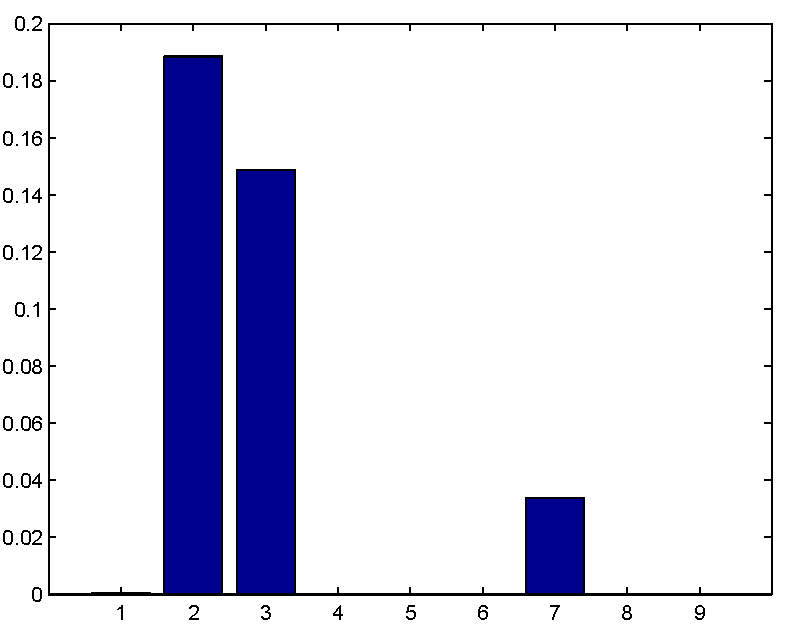
\includegraphics[width=0.4\textwidth]{../diagrams/supplMocapScalesRbf}
	\label{fig:suppMocap1}
}
\subfigure[]{
	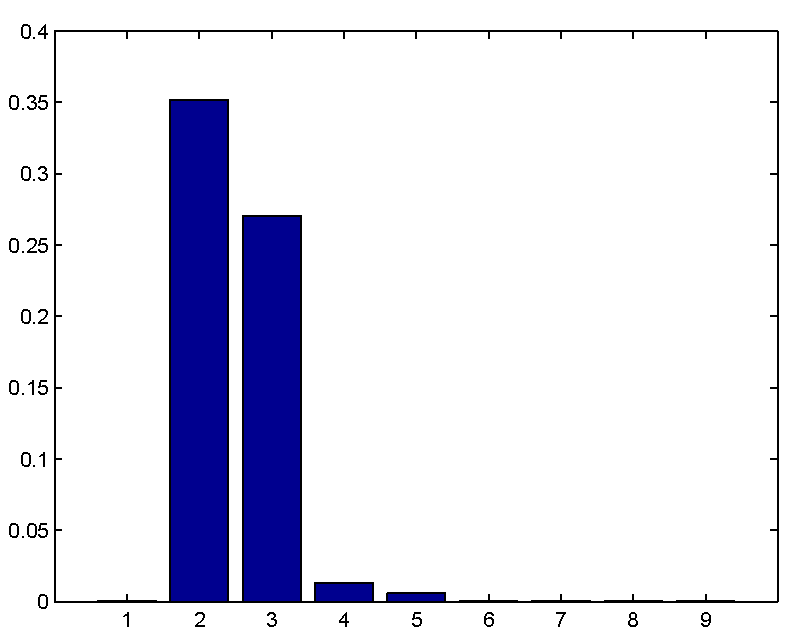
\includegraphics[width=0.4\textwidth]{../diagrams/supplMocapScalesMatern}
	\label{fig:suppMocap2}
}
\end{center}
\caption{\small{
The values of the scales of the ARD kernel after training on the motion capture dataset using the RBF (fig: \subref{fig:suppMocap1}) and the Mat\'ern (fig: \subref{fig:suppMocap2}) covariance function to model the dynamics for VGPDS. The scales that have zero value ``switch off'' the corresponding dimension of the latent space. The latent space is, therefore, 3-D for \subref{fig:suppMocap1} and 4-D for \subref{fig:suppMocap2}. Note that the scales were initialized with very similar values.
}
}
\label{fig:supplMocap1}
\end{figure}


\begin{figure}[ht]
\begin{center}
\subfigure[]{
	%\includegraphics[width=0.48\textwidth]{../diagrams/supplMocapBody23GpdsRbf}
	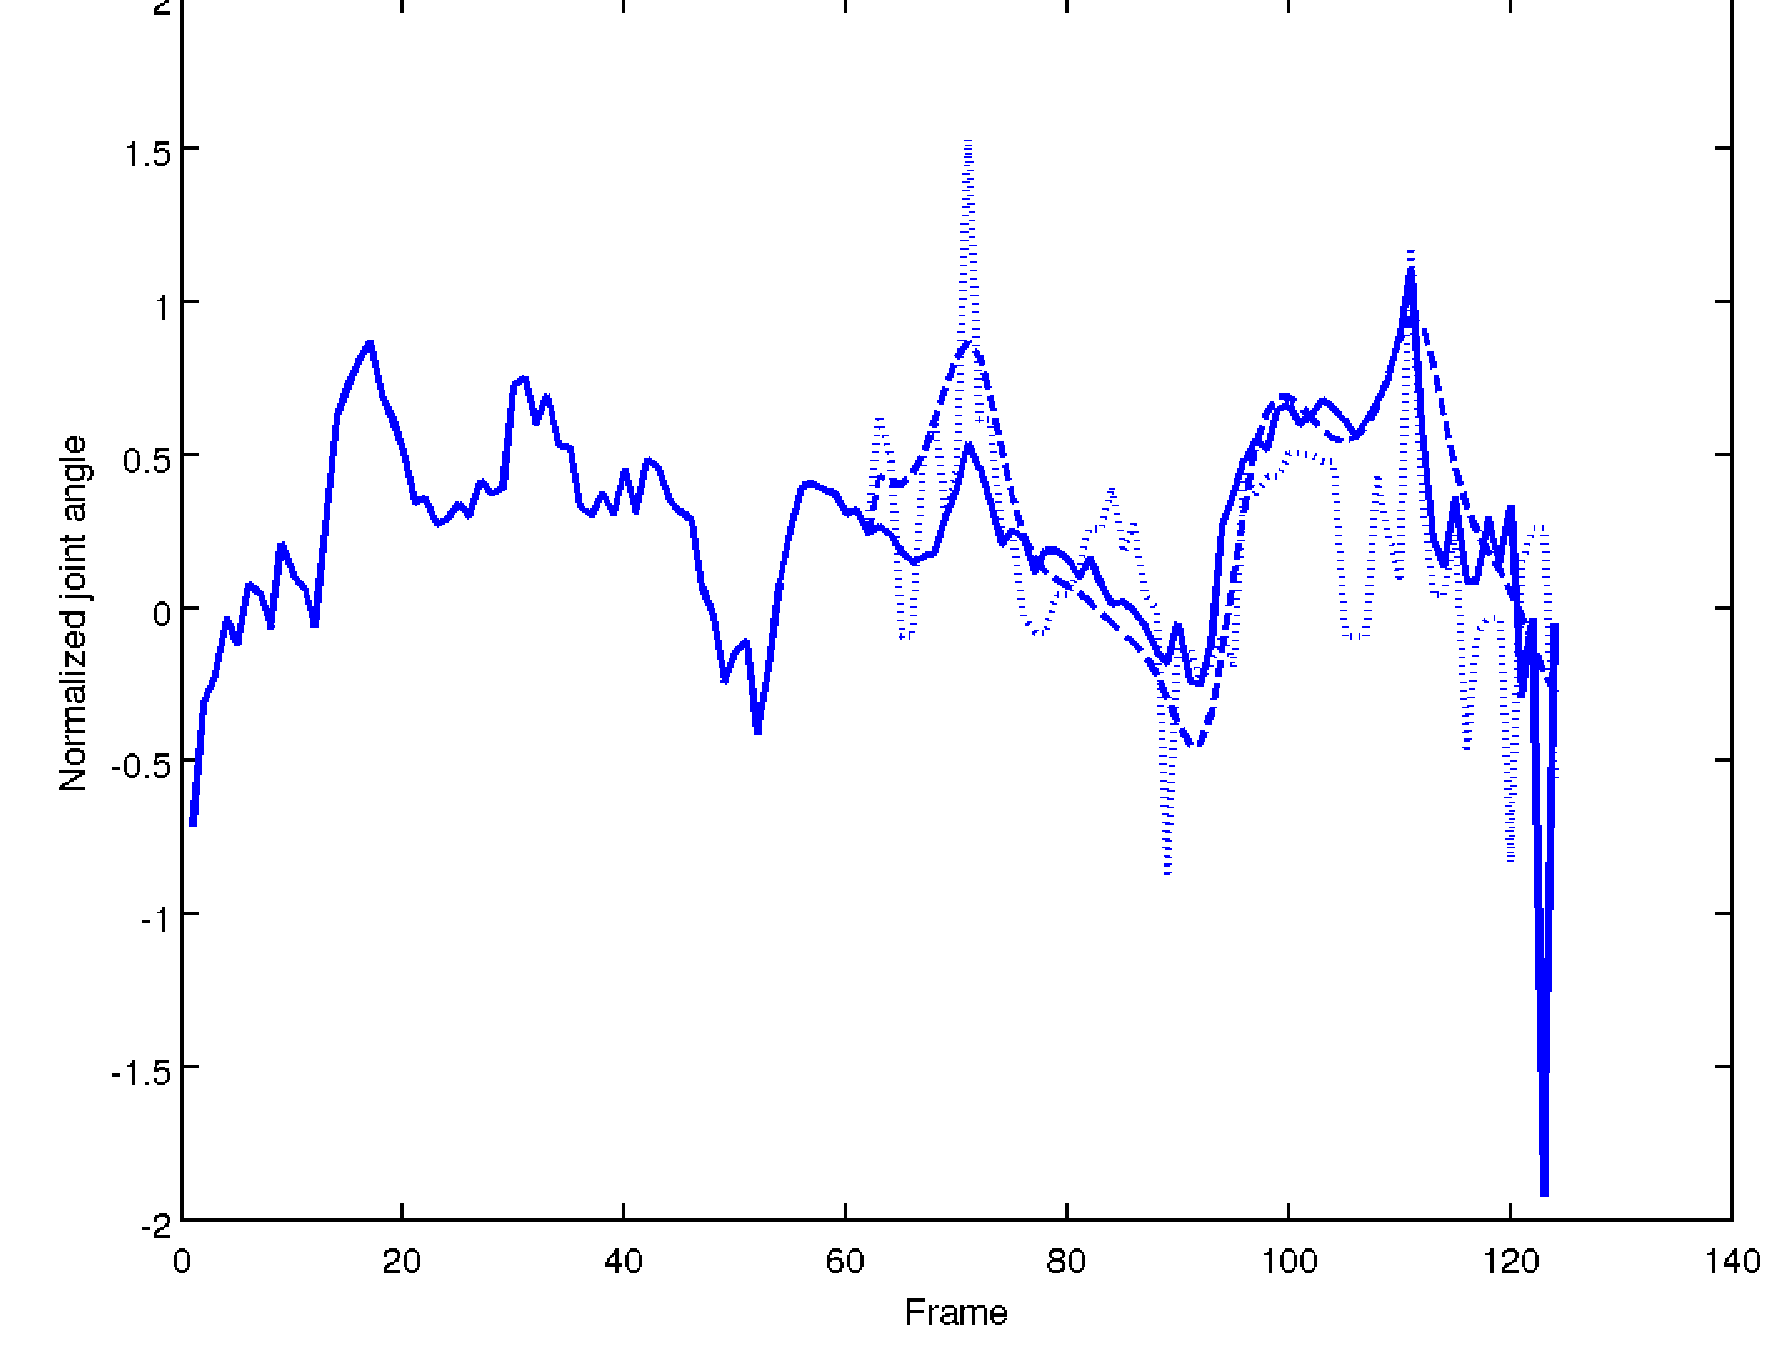
\includegraphics[width=0.48\textwidth]{../diagrams/supplMocapBody28GpdsMatern}
	\label{fig:suppMocap3}
}
\subfigure[]{
	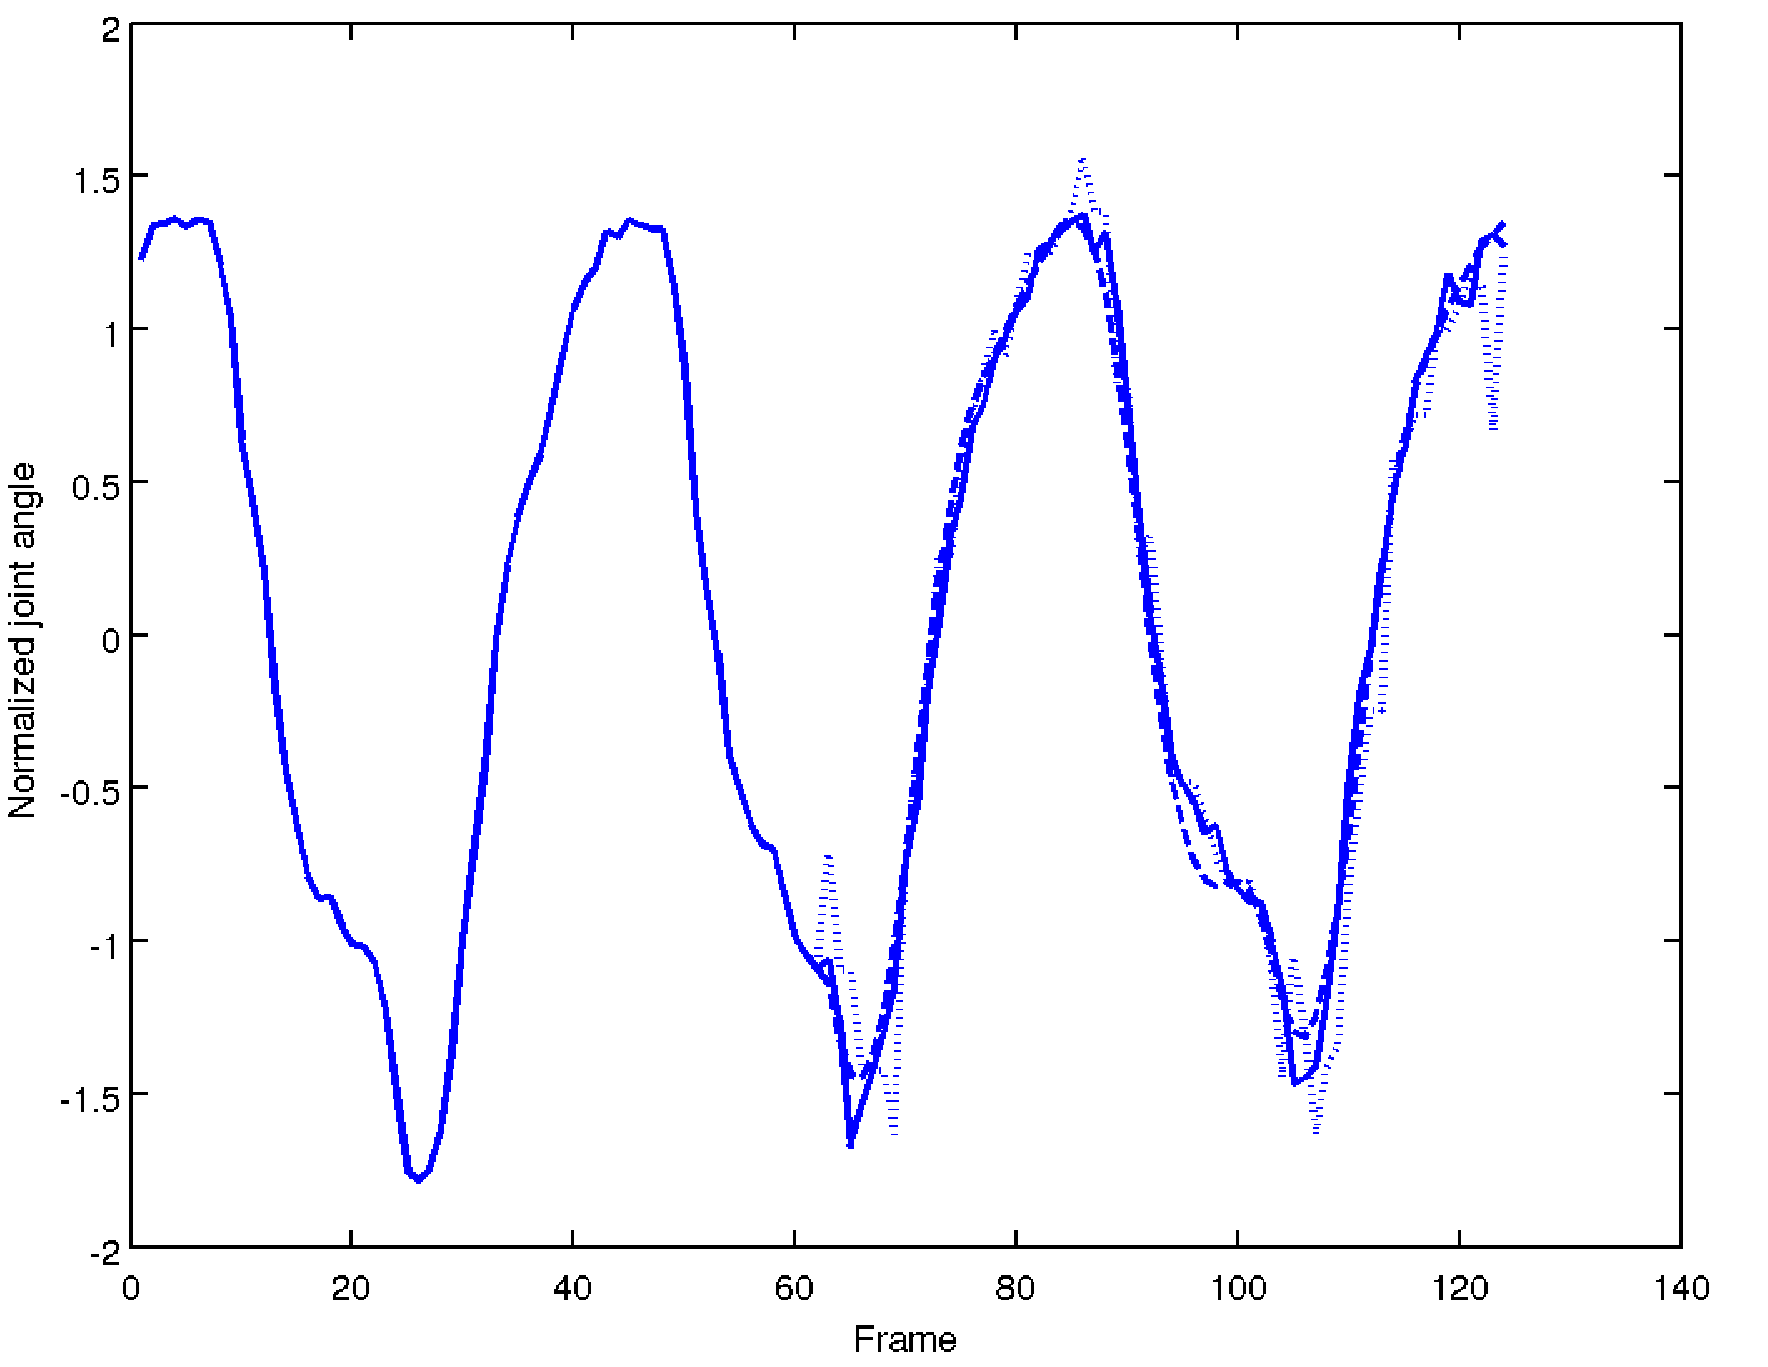
\includegraphics[width=0.48\textwidth]{../diagrams/supplMocapLeg5GpdsMatern}
	\label{fig:suppMocap4}
}
\end{center}
\caption{\small{
The prediction for two of the test angles for the body (fig: \ref{fig:suppMocap3}) and for the legs part (fig: \ref{fig:suppMocap3}). Continuous line is the original test data, dotted line is nearest neighbour in scaled space, dashed line is VGPDS (using the RBF covariance function for the body reconstruction and the Mat\'ern for the legs).
}
}
\label{fig:supplMocap2}
\end{figure}




\begin{figure}[ht]
\begin{center}
\subfigure[]{
	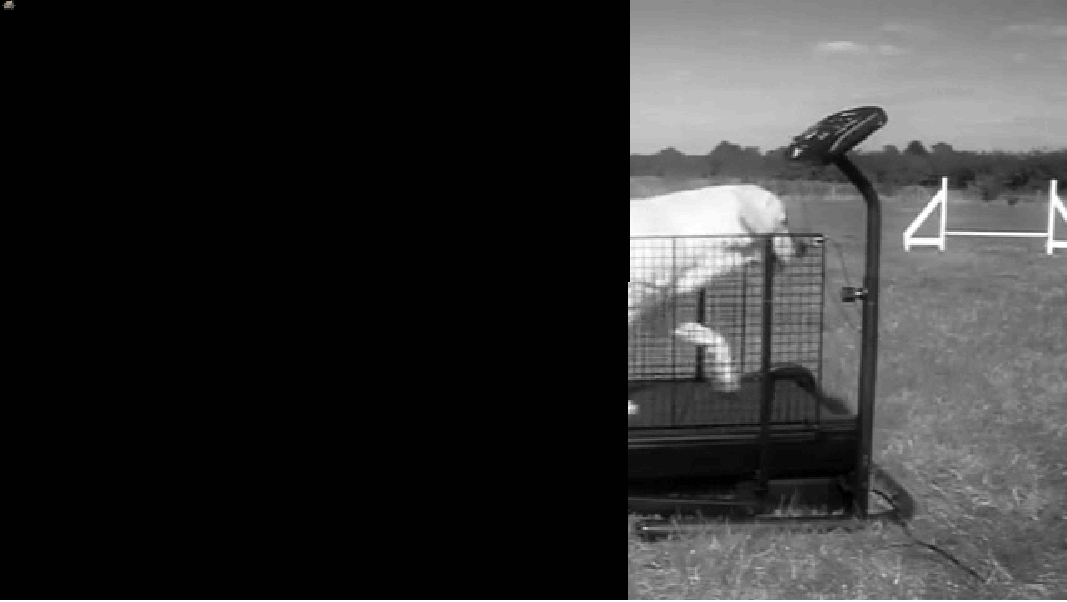
\includegraphics[width=0.23\textwidth]{../diagrams/supplDogPredYts5}
	\label{fig:suppDog1}
}
\subfigure[]{
	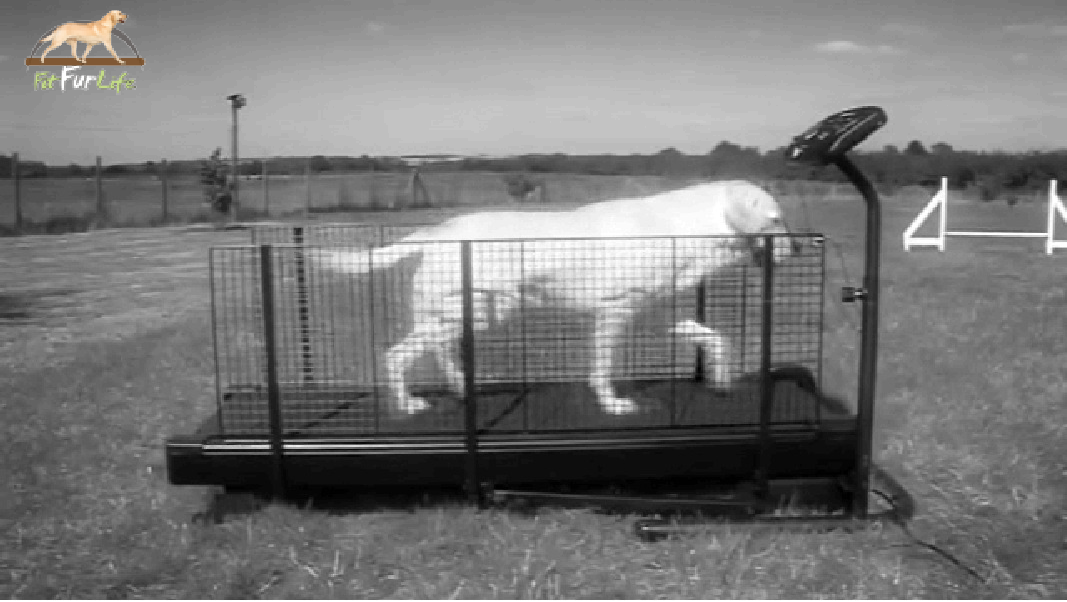
\includegraphics[width=0.23\textwidth]{../diagrams/supplDogPredGpds5}
	\label{fig:suppDog2}
}
\subfigure[]{
	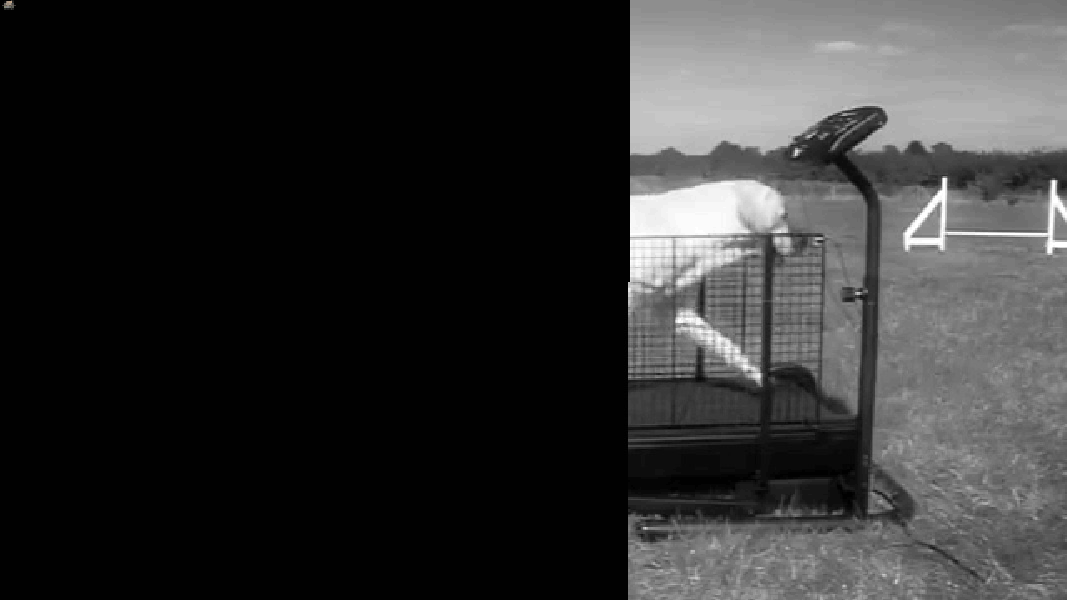
\includegraphics[width=0.23\textwidth]{../diagrams/supplDogPredYts6}
	\label{fig:suppDog3}
}
\subfigure[]{
	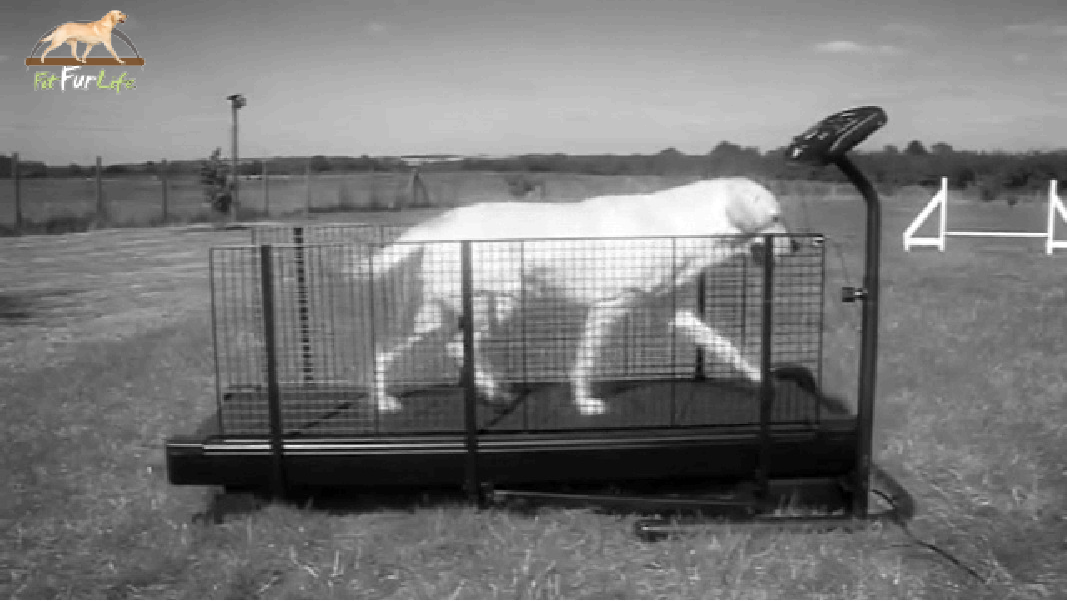
\includegraphics[width=0.23\textwidth]{../diagrams/supplDogPredGpds6}
	\label{fig:suppDog4}
}
\end{center}
\caption{\small{
 Some more examples for the reconstruction achieved for the `dog' dataset. $40\%$ of the test image's pixels (figures \subref{fig:suppDog1} and \subref{fig:suppDog3}) were presented  to the model, which was able to successfully reconstruct them, as can be seen in \subref{fig:suppDog2} and \subref{fig:suppDog4}.
}
}
\label{fig:supplDog}
\end{figure}
